\chapter{Développement d'un jeu} % (fold)
\label{cha:développement_d_un_jeu}

Dans ce chapitre, je vais parler du développement du jeu <<Playboy-spots>>. <<Playboy-spots>> est le premier jeu que j'ai participé dans ma vie. Au début jusqu'au produit finale. Pendant ces processus de développement, j'ai appris beaucoup de chose, concept etc. Non seulement que j'ai appris beaucoup, mais aussi, grâce à ce projet, j'ai commencé à réfléchir beaucoup, comparer les techniques utilisés, résumer les points négative et positive. Ces expérience vont m'aider beaucoup dans les projets futurs. Dans n'importe quelle entreprise.

\section{Processus} % (fold)
\label{sec:processus}

Un jeu est un logiciel spéciale. Au niveau de ressource, un jeu est plus difficile à développer par rapport aux logiciel. Parce que un jeu demande beaucoup de ressource par rapport aux logiciels. Je vais le parler dans section suivant. Au niveau de processus de développement. Un jeu est plus simple par rapport aux logiciel. Ici, je vais parler le processus de développement d'un jeu en général et en comparant avec le processus réel chez chugulu games. surtout, il faut savoir, ici, le processus est utilisé par les petites équipes. Pour les grandes entreprises comme <<EA>>, ils ont un autre processus plus complet, plus systématiques, mais va durer plus long, et leurs processus est utilisé pour créer des jeux gros. Pour chugulu games et billions des studio comme chugulu games, leurs caractéristiques commune sont petite, bouger simple, réactiver rapide, développer rapide. 

\subsection{Processus Général} % (fold)
\label{sub:processus_général}

En générale, au niveau de programmation, le processus général n'est pas très loin que la processus classique d'un logiciel. Le processus peut être décomposé en plusieurs étape, qui sont présentés dans le schéma comme figure~\ref{fig:XMinds_Gamedevelopement}.

% TODO add schéma générale
\begin{figure}[htbp]
	\centering
		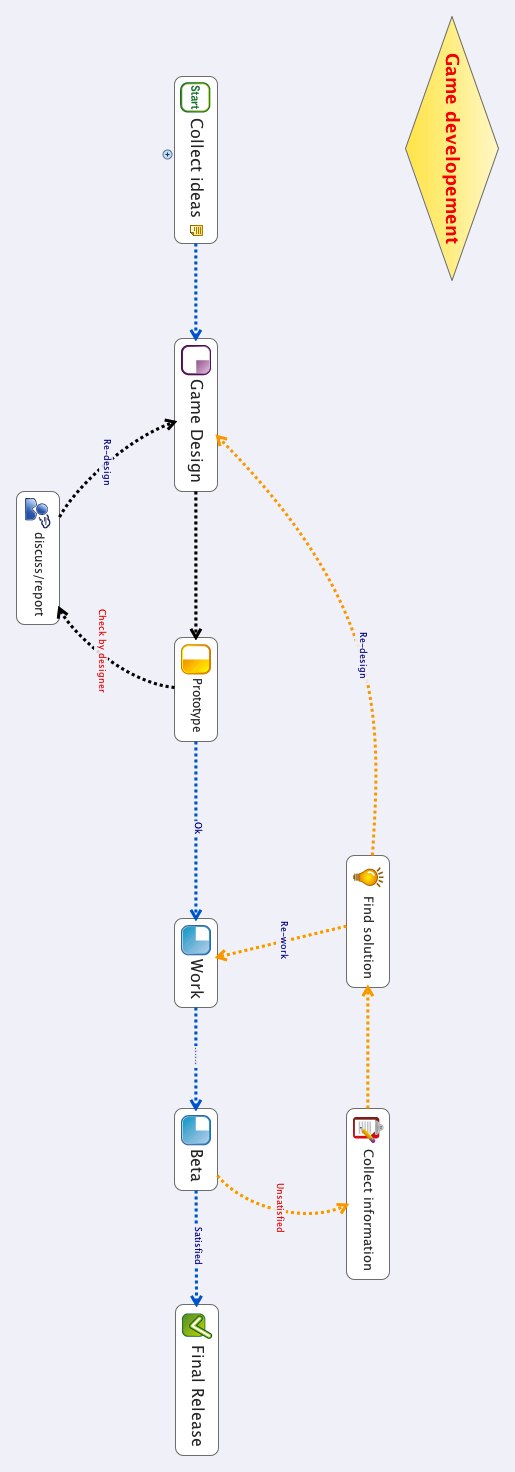
\includegraphics[height=9in]{XMinds/Gamedevelopement.png}
	\caption{caption}
	\label{fig:XMinds_Gamedevelopement}
\end{figure}

Dans ce figure, on peut voir, généralement, un développement du jeu peut être divisé en les étapes suivantes :

\subsubsection{Collect ideas} % (fold)

Développer un jeu peut avoir plusieurs raison. Peut être, nous avons trouvé des idées très intéressantes. Peut-être, nous avons trouvé que dans la marché du jeu, il manque ce genre de jeu, donc, le jeu ce que nous faisons va être réussis dans la futur. Peut-être, nous allons regarder un jeu qui est déjà réussis, qui a vendu billiard euros, et nous décidons de juste créer un jeu qui ressemble, mais en même temps, plus <<Intelligent>>. Peut-être, peut-être... Nous avons mille d'excuse pour créer un jeu. Pareil, selon les type de jeu, selon l'entreprise, nous pouvons avoir plusieurs processus totalement différent pour créer un jeu. 

Mais, dans toutes les processus différente, il existe un étape commune, essentiel et importante. C'est l'étape de collection des idées. 

Cet étape signifie à définir un principe du jeu en générale. Après cet étape, nous devons être sure que, notre jeu doit afficher quoi, comment jouer notre jeu. Donc, dans cet étape, ce que nous nous discutons est la chose la plus importante. 

Un autre point à savoir, c'est que, dans cet étape, souvent, nous savons pas les interfaces doivent afficher comment. Dans cet étape, souvent, une entreprise va organiser plusieurs réunions.

Dans le jeu de <<Playboy-Spots>>, dans cet étape, nous avons réussi a déterminer la coeur du jeu. Par exemple, nous savons que, nous avons plusieurs pack, chaque pack contient certaines photos. Nous savons que, sur chaque photo, il y aura certaine différences à trouver. Le nombre des différence n'est pas fixé, peut être 5, peut être 4. Nous savons que, nous avons 3 mode de jeu, sur chaque mode, le jeu va être joué différemment etc..

% subsubsection Collect ideas (end)

\subsubsection{Game Design} % (fold)

Dans cet étape, les game désigners vont commencer désigner le jeu. Concernant n'importe quel élément dans le jeu. Game désigners vont essayer de déterminer toutes les interfaces, les mécanismes (par exemple, les mécanisme de scoring, etc.) Les désigners vont essayer de sortir toutes les mock-up sur toutes les interfaces. 

En fait, cet étape est un début d'un cycle. Ce cycle commence par game désign, ensuite, les développeurs vont essayer de sortir une prototype, et à la fin, les développeurs vont montrer le prototype aux game désigners pour qu'ils puissent regarder ce qui donne, puissent savoir s'il y a des problème au niveau de conception, mécanisme, etc. Ce cycle peut durer longtemps, puisque, un jeu n'égale pas à un logiciel. Nous ne savons pas si nos désignes sont bonne ou pas, intéressantes ou pas. Donc il est essentiel de regarder notre idée devient réel, et jouer en réel. S'il y a des choses qui ne marchent pas, nous pouvons avoir de la chance de corriger avant commencer à programmer.

Normalement, après cet étape, nous devons être capable de sortie un cahier qui décrit toutes nos designs pour que nous puissions commencer développer.

% subsubsection Game Design (end) 

\subsubsection{Prototype} % (fold)

Dans les petite entreprise, ou les petits studios, cet étape est important. Souvent, dans ce cas, nous n'avons pas beaucoup de développeur, ni beaucoup de temps. Souvent, les jeux que nous allons développé ne sont pas gros. Ils sont les petite jeux. Il est possible de créer les prototypes dans ces cas. 

Un prototype est défini pas wikipédia comme suivante : Un prototype désigne le premier, ou l'un des premiers exemplaires d'un produit industriel (voiture, avion…). Cet exemplaire permet de faire des tests afin de valider les choix de conception de l'ensemble. Le prototype précède les exemplaires de pré-série. 

Dans le développement du jeu, notre prototype va déterminer le structure du jeu, les fonctionnalités générales dans le futur. 

% subsubsection Prototype (end)

\subsubsection{Work} % (fold)

Quand nous allons dans cette étape, nous somme sure que toutes les désigns sont déjà fait, validé par game désigner. Il n'existe pas grand problème dans prototype. Nous avons bien déterminer les éléments du jeu. Donc, nous pouvons commencer développer. 

Cette étape va duré longtemps, tous membres dans l'équipe vont rejoindre dans ce projet. En même temps, toutes les autre équipe vont commencer à travailler, par exemple l'équipe de graphiste, l'équipe de musique etc.. 

En fait, cette étape peut être divisé en plusieurs sous étapes. Prendre le programmation comme exemple, nous pouvons décomposé en plusieurs comme <<Faire la cahier de charge>>, <<Construire la structure général>>, etc..

% subsubsection Work (end)

\subsubsection{Beta} % (fold)

L'étape suivant est l'étape de Beta. Dans cette étape, normalement, nous avons bien développé notre jeu. Même s'il y a beaucoup des bugs, des erreurs, des fonctionnalités qui ne marchent pas. Le but de cette étape est de tester s'il y a gros problème à corriger. Non seulement les bugs qui font crasher le jeu, mais aussi les designes qui n'a pas l'air bien et utile. Dans ces 2 cas, il faut que nous collectons tous des informations nécessaires, trouvons des solutions, et donner aux développeurs ou désigners de soit corriger les bugs soit redésigner. 

Cette étape peut se répète plusieurs fois. En fait, aucun jeu peut être publié directement après développement. Ce n'est pas du tout possible. Il est normale d'avoir plain de bugs dans un jeu. Le jeu le plus complexe demande le plus de temps dans cette étape. Surtout le jeu en ligne comme <<World of Warcraft>>. Il avait fait 6 mois de beta public, c-à-d demande de joueur à jouer. Et avant ce commencer le beta public, il a déjà fait assez longtemps de beta test. Nous ne pouvons pas savoir précisément combien de temps a passé à l'interne de <<World of Warcraft>>, mais nous somme sur que cette étape est assez long. 

Il est pareil pour <<Playboy-Spots>>. Nous avons terminer le développement du jeu vers mi-aout, les reste du temps jusqu'à final, ne comporte que deux tâches. Une est débug, test le beta, corriger, une autre est amélioration. 

Amélioration est importante pour un jeu ou un logiciel. Souvent, il est pas si grave si un logiciel qui n'est pas amélioré. Sauf le logiciel très professionnel. En revanche, l'amélioration est souvent très grave pour un jeu. C'est à cause du complexité du jeu par rapport au logiciel. Et aussi le structure spécial du jeu. Un jeu peut prendre beaucoup de ressource du système, s'il n'est pas améliorer. C'est parce que un jeu comporte souvent un intelligent artifice complexe qui demande beaucoup de calcul. Un jeu comporte beaucoup des image, des son à afficher. Si ce jeu est un jeu 3D, il va prendre beaucoup plus de temps pour <<render>> des objets 3D sur l'écran. Souvent, un jeu est strictement besoin de fluide. 

L'amélioration peut comporte plusieurs aspects. Au niveau de mémoire, au niveau des ressource, au niveau de algorithmes, au niveau d'affichage, etc.. Les façons d'amélioration peut comporte beaucoup des façons différente aussi selon ce que nous allons améliorer. Elles peuvent être modifier les formats des images, remplacer les fonctions du système, utiliser multi-threading, utiliser multi-core, etc..

Dans <<Playboy-Spots>>, nous avons travaillé beaucoup sur améliorations. Y compris le fluide dans la boutique, diminue le temps de charge pour un jeu, diminue les mémoire consumé, etc.. 

% subsubsection Beta (end)

\subsubsection{Final release} % (fold)
\label{ssub:final_release}

C'est la dernière étape d'un cycle du produit. Ici, je vais parler principalement sur App Store d'apple. App Store est une boutique de logiciel créée par Apple. Cette boutique n'est utilisée dans les équipements iOS. Ce sont les équipements iPhone, iPad et iPod Touche. Apple a crée cette boutique depuis 2008, et aujourd'hui, elle est la meilleur boutique du monde sur les mobiles. Et aussi, grace à cette boutique, il peut avoir milliard des applications pour les utilisateurs. Cette année, apple a ouvert la deuxième boutique, qui est crée spécialement pour Mac OS, qui s'appelle Mac Store. 

Aujourd'hui, il y a de plus en plus de développeur ont commencé crée leurs applications et les publiés sur App Store. En fait, la boutique App Store est la seule façon légal pour publier et vendre une application sur un équipement iOS. Pareil pour chugulu games. Une fois <<Playboy-Spots>> a été fini améliorations, test, etc. Nous pouvons le publier sur App Store. Ce processus pour publier une application sur App Store n'est pas du tout facile. Dans ce processus, souvent, Apple va examiner notre application. Si notre application a trop de bugs, mal désigné d'interface, mal fonctionne, inutile etc.. Apple va rejeter notre application.

% subsubsection final_release (end)

% subsection processus_général (end)

\subsection{Processus chez Chugulu Games} % (fold)
\label{sub:processus_chez_chugulu_games}

Chez chugulu games, nous somme dans un cas particulière. Comme indiquer précédente, le processus de développement du jeu est varié selon le type du jeu. Les jeux développés par chugulu games peuvent être divisé en 3 gros catégories : 

\begin{description}
	\item[Edition] Un jeu d'édition est un jeu annoncé par chugulu, désigné par chugulu et publié par chugulu. Ce type du jeu est développés totalement par chugulu.
	\item[Co-edition] Un jeu de co-edition est souvent annoncé par une autre entreprise. Chugulu développe ce jeu avec telle entreprise. Ce jeu peut être désigné par autre entreprise, chugulu ne se charge que le développement. Par exemple, <<Playboy-Spots>> est un jeu de co-edition, il est annoncé par entreprise <<1663sa>>. <<1663sa>> se charge de désigner, chugulu se charge de développement. Dans l'application finale, il y aura un crédit qui contient les membres de chugulu et 1663sa.
	\item[Prestation] Un jeu de prestation est un jeu annoncé par une autre entreprise, qui n'est pas une entreprise d'informatique souvent. Chugulu négocier avec cette entreprise pour savoir ses besoins. Et chugulu donner un jeu finale au cette entreprise. Ce jeu est développé par chugulu totalement, désigné par chugulu aussi. La seule différence entre ce type et type <<Edition>> est que, ce type de jeu doit respecter les besoins.
\end{description}

Au niveau de processus, les types <<Edition>> est exactement pareil comme le processus général. Donc, ici, je vais me concentrer sur les autres types, <<Co-edition>> \& <<Prestation>>

% TODO add processus chugulu games

\begin{figure}[htbp]
	\centering
		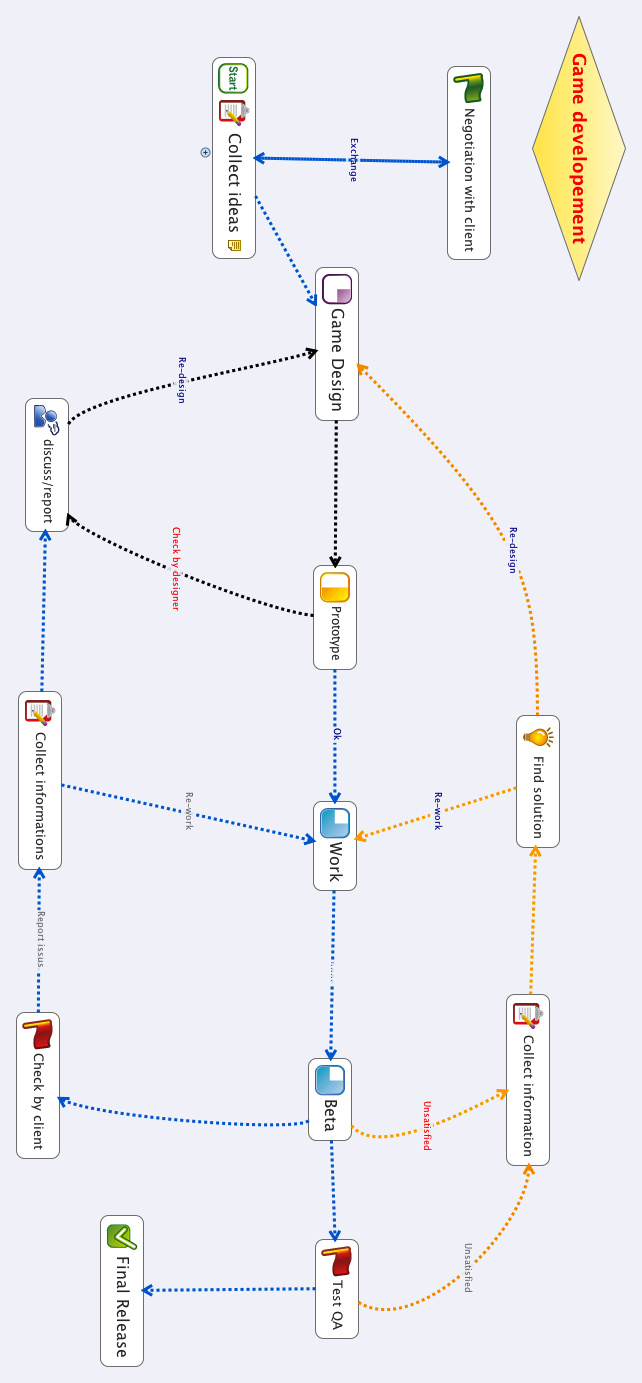
\includegraphics[height=9in]{XMinds/GamedevelopementChugulu.png}
	\caption{caption}
	\label{fig:XMinds_GamedevelopementChugulu}
\end{figure}


Sur ce schéma, nous pouvons savoir que, ce processus n'est pas très différente par rapport au processus général. En résumant les différences, elles sont principalement des étapes avec des drapeaux dessus. 

\subsubsection{Negotiation with client } % (fold)
\label{ssub:negotiation_with_client_}

Tout début, juste après annoncé par des autre client. Il existe une étape pour négocier avec le client. Cette étape sert à savoir les besoins ou les charges. Si ce jeu est un type de <<Prestation>>, il est obligé de passé certaines temps pour savoir les besoins du clients, et échanger nos idée avec le client. Pareil pour le type du jeu <<Co-edition>>, il faut non seulement échanger nos idée, mais aussi diviser les charges. Il faut définir que qui va se charger de désigner le jeu, qui va se charger de développer ce jeu.

% subsubsection negotiation_with_client_ (end)

\subsubsection{Check by client} % (fold)
\label{ssub:check_by_client}

C'est une autre étape différente par rapport au processus général, qui s'appelle <<Check by client>>. Cette étape se situe souvent à la fin des développement, se répète plusieurs fois jusqu'à la fin de l'étape <<Beta>>. 

Cette étape ressemble à l'étape de <<Beta>>. Dans cette étape, nous somme obligé de passé notre application au client. Le client va l'examiner pour voir s'il y a de chose qui ne va pas.

% subsubsection check_by_client (end)

\subsubsection{Test QA} % (fold)
\label{ssub:test_qa}

Test QA est une étape importante chez chugulu. En fait, test QA est <<Beta>> test par les joueurs public. Chugulu games va publier un jeu, par exemple, <<Playboy-Spots>> vers certaine joueurs. Inséré des fonctionnalité qui permet de reporter toutes les status, les bugs, vers un site web. Grace à cela, nous pouvons savoir les problèmes graves et trouver les solutions.

Test QA est utilisé souvent par chugulu games.  

% subsubsection test_qa (end)

\section{Équipe} % (fold)
\label{sec:Équipe}
% subsection processus_chez_chugulu_games (end)

% section processus (end)

\subsection{Strucutre d'équipe chugulu} % (fold)
\label{sub:strucutre_d_équipe_chugulu}

% TODO  add équipe de chugulu

\begin{figure}[htbp]
	\centering
		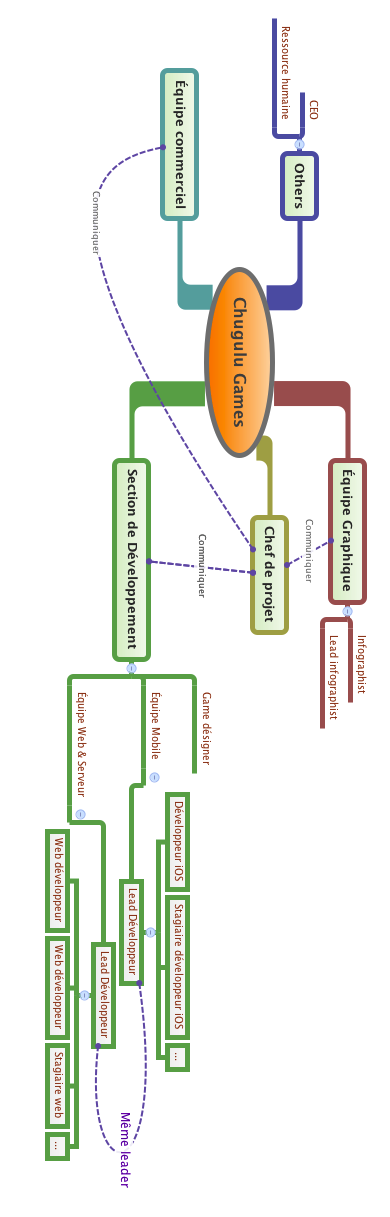
\includegraphics[height=9in]{XMinds/EquipeChuguluGames.png}
	\caption{caption}
	\label{fig:XMinds_EquipeChuguluGames}
\end{figure}


Chugulu games a deux poste du monde. Le poste principale est à Paris, qui se charge de développement, de communiquer avec clients et etc.. Le poste des état-unis ne se charge que maintenir et publier les jeux Edition de chugulu. Ici, je vais parler seulement de l'équipe à Paris, qui représente une structure générale et traditionnelle.

Un jeu est un logiciel spéciale comme indiqué dans les chapitres précédente. Pour créer un jeu, il faut demander plusieurs ressource variée, il faut des spécialistes de différente sections travaillent ensemble. Un jeu a besoin de graphistes, de développeurs, de musiques créateurs, de commercial, de game désigner, de réalisateurs etc.. Cependant, un logiciel peut n'avoir besoins que des développeurs.  

Sur ce schéma, nous pouvons remarquer que, chugulu a 4 équipe en générale. Ils sont : 
\begin{description}
	\item[Equipe Graphiste] Une équipe qui se charge de créer des graphiques. 
	\item[Equipe Mobile] Une équipe qui se charge de créer des applications sur l'équipement iOS.
	\item[Equipe Web \& Serveur] Une équipe qui se charge de créer des jeux sur des site web comme Facebook etc..
	\item[Equipe commercial] Cette équipe se charge de communiquer avec les client, publier les nouveauté, etc..
\end{description}
Sauf les 4 équipes, chugulu a aussi certaines comme les autres entreprise, comme CEO, ressource humaine, chef de projet, game désigner etc..

Il est très important d'avoir communication parmi les 4 équipes. Souvent, c'est grace à chef de projet, qui communiquer les différentes équipes. 

% subsection strucutre_d_équipe_chugulu (end)

\subsection{Structure d'équipe mobile et les responsabilités} % (fold)
\label{sub:structure_d_équipe_mobile_et_les_responsabilités}

\begin{figure}[htbp]
	\centering
		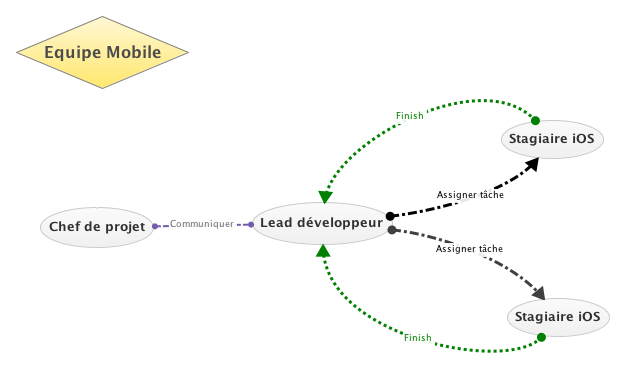
\includegraphics[width=6in]{XMinds/EquipeMobile.png}
	\caption{caption}
	\label{fig:XMinds_EquipeMobile}
\end{figure}


L'équipe mobile de chugulu games a comporte de un lead ios développeurs et 2 ios développeur stagiaires. L'équipe mobile de chugulu est quand même une équipe très jaune. Le lead iOS développeur est partagé par l'équipe mobile et l'équipe web. Moi et un autre stagiaires, nous somme les 2 autre développeurs. 

Au niveau de responsabilités, le lead ios développeurs se charge de décider toute l'architecture du jeu, découpé les tâches, et assigner les tâches à nous. Sauf ci, il développe avec nous, communique avec le chef de projet, essayer de trouver des solutions pour les problèmes que nous rencontrons pendant les travails. Le processus chez chugulu peut être représenter par un schéma suivant comme le Figure~\ref{fig:XMinds_ProcessusMobile}:

\begin{figure}[htbp]
	\centering
		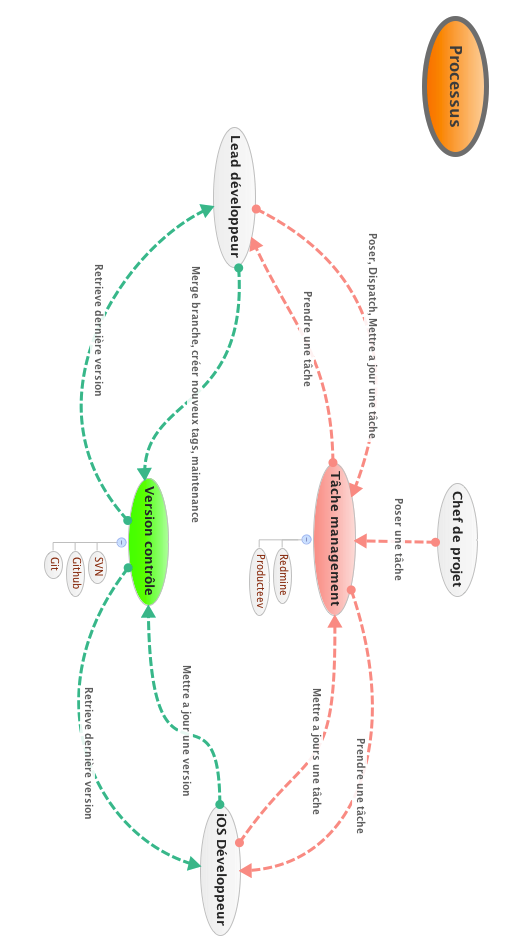
\includegraphics[height=9in]{XMinds/ProcessusMobile.png}
	\caption{caption}
	\label{fig:XMinds_ProcessusMobile}
\end{figure}


À partir de ce schéma, nous pouvons remarquer que, nous avons 2 outils principaux. Un outil est l'outil pour manager les tâches. C'est ce que j'ai raconté précédente : Redmine ou Producteev. Un autre outil est l'outil pour contrôler les versions, ils sont : SVN, Git, et un site accompagne avec Git : github. 

Souvent, chef de projet ou lead développeur, ils poser uns ou plusieurs tâches sur redmine. Ensuite, lead développeur peut assigner une ou plusieurs tâches à un développeur. Lui et les développeurs vont commencer regarder toutes les tâches. Il faut travail en suivant l'ordre de priorité. Prendre la tâche la plus grave. Il faut mettre à jours le status sur redmine, ainsi que les résultats ou les tips. Une fois une tâche soit fini, nous devons mettre à jours notre version par Git ou Svn. Nous mettre à jours notre dernière code, résoudre les confits, etc.. Le lead développeur va prendre la dernière version, examiner, merge et mettre à jours le repositoire.


% subsection structure_d_équipe_mobile_et_les_responsabilités (end)

% section Équipe (end)

\section{Structure} % (fold)
\label{sec:structure}

Un jeu est un logiciel différente. Non seulement son fonctionnalité, son but, mais aussi son structure. Un structure est souvent liée avec ses fonctionnalité, et façon de fonction. 

\subsection{Le structure général d'un jeu} % (fold)
\label{sub:le_structure_général_d_un_jeu}

Un jeu peut souvent bouger lui même sans l'activité des joueurs. C-à-d que, quand tu ne donne pas tes instructions, tes commands, le jeu peut bouger quand même. Il peut afficher une animation, il y a des objets qui bougent, le temps passé, des <<Civils>> se chats etc.. C'est parce que un jeu est dans quelque niveau un simulation d'un environnement. Un jeu toujours essaie de simuler un environnement vivant. Dedans, les joueurs peuvent avoir une impression que ils sont une membre qui appartient au environnement. Et ils peuvent avoir envie de interagir avec les objets, avec l'environnement, même si cet environnement n'est pas vrai. Tout cela est un facteur hyper importante pour un jeu qui veut être réussit.

Le Figure~\ref{fig:XMinds_MainGameLoopAchitecture} represente ce structure générale


\begin{figure}[htbp]
	\centering
		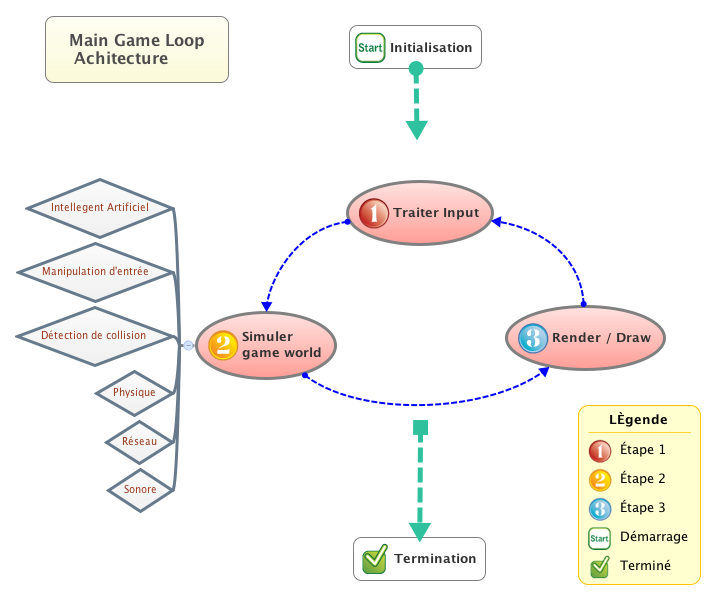
\includegraphics[width=6in]{XMinds/MainGameLoopAchitecture.png}
	\caption{caption}
	\label{fig:XMinds_MainGameLoopAchitecture}
\end{figure}

À partir de ce schéma <<Game loop>>, nous pouvons savoir, il y a 3 étape générale dans un game loop. Souvent, un jeu commence par étape <<Initialisation>>. Dans cette étape, le joueur va choisir les options, mode à jouer, etc. Une fois, le joueur clique sur <<Jouer>>, notre game loop commence à rouler. Souvent, un game loop commence par attendre l'input du joueur. Si un joueur n'input pas, game loop va aller dans l'étape 2, qui s'appelle <<Simuler game world>>. Dans cette étape, le jeu va essayer de simuler l'environnement du jeu par rapport aux inputs du joueurs. Ce simulations dépends sur les règles que nous avons donner. Précisément dire, nous pouvons avoir des règles comme <<Intellegent Artificiel>>, <<Collision detect>> etc.. Après cette étape, nous obtenons les résultats et l'environnement prêt à dessiner. C'est le moment où on dessiner les environnements dans l'écran devant le joueur.

Je vais parler des étapes :

\subsubsection{Game Loop} % (fold)
\label{ssub:game_loop}

Le gameplay sera exécuté dans une boucle. Les principaux composants de cette boucle sera Update et Draw. La boucle sera nécessaire pour faire fonctionner soixante fois par seconde.

\subsubsection{Draw} % (fold)
\label{ssub:draw}
Draw sera responsable pour le dessin à l'écran en fonction de variables d'état différents. La vue sera tributaire de la position du joueur, l'orientation et la vitesse. Options de la caméra de l'utilisateur sera également affecter la vue. Il y aura un appel Draw pour chaque appel Update.
% subsubsection draw (end)

\subsubsection{Simuler de l'environnements/mise à jour} % (fold)
\label{ssub:subsubsection_name}

Simuler de l'environnements sera responsable de tous les changements d'état de jeu n'est pas liée à dessin. Il s'agira notamment AI, entrée, détection de collision, de mouvements d'objets (physique), réseau et audio.


% subsubsection game_loop (end)

\subsubsection{Intelligent Artificiel } % (fold)
\label{ssub:a_i_décisions_}
Durant cette phase de la mise à jour, A.I. prend les décisions sur l'endroit où aller, comment dépenser les crédits pour moderniser leurs navires, ce qui à feu à et quelle arme à utiliser. 

Les décisions ne peuvent être faites lors de chaque appel de Update. A.I. mises à jour peut être reporté à améliorer les performances.

% subsubsection a_i_décisions_ (end)

\subsubsection{Manipulation d'entrée} % (fold)
\label{ssub:manipulation_d_entrée}

Durant cette phase de la mise à jour, toutes les informations de l'utilisateur seront analysées et traitées. Toutes les commandes validés seront exécutées immédiatement. Toutes les commandes invalides retour à l'utilisateur ou tout simplement être jetés hors basé sur la commande et de la situation. 

Manipulation d'entrée sera fait à chaque cycle  pour s'assurer que le jeu semble réceptif à tout moment.

% subsubsection manipulation_d_entrée (end)

\subsubsection{Détection de collision} % (fold)
\label{ssub:détection_de_collision}

Durant cette phase de la mise à jour, tous les objets va vérifier si elles entrent en collision avec d'autres objets. Partitionnement spatial sera utilisé pour améliorer les performances de ces contrôles. Si une collision se produit, le système de détection de collision va coopérer avec le système physique pour déterminer les forces appropriées à appliquer à chaque objet. Dommage, les crédits et appropriée des effets graphiques peuvent également avoir besoin d'être appliquée. 

Détection de collision se produira à chaque cycle.

% subsubsection détection_de_collision (end)

\subsubsection{Physique} % (fold)
\label{ssub:physique}

Durant cette phase de la mise à jour, tous les objets seront déplacés en fonction de leurs mouvements et de composants vitesse de rotation. Le mouvement et les composantes de vitesse de rotation sera également mis à jour pour refléter toutes les forces appliquées à l'objet. 

Physique sera effectué à chaque cycle.

% subsubsection physique (end)

\subsubsection{Réseaux} % (fold)
\label{ssub:réseau}

Durant cette phase de la mise à jour, toutes les fonctions de réseaux seront traitées. Le but de la mise en réseau sera de synchroniser les «univers». Il s'agira notamment de l'envoi de toutes les données sur le vaisseau du joueur et les projectiles, ainsi que de recevoir les mêmes données à d'autres joueurs. 

Réseaux ne se fera pas à chaque cycle jour. Réseaux sera reporté au besoin, pour améliorer les performances. Réseaux ne sera pas présent dans les jeux solo.

% subsubsection réseau (end)

\subsubsection{Sonore} % (fold)
\label{ssub:sonore}

Sonore sera spéciale que des autres phases du cycle de mise à jour. Il ne sera pas traitée dans la boucle de mise à jour, seulement instancié. La méthode mise à jour sera responsable de décider quand les sons doivent être joués en fonction des événements dans le jeu. Toutes les sons réels seront traitées par les threads qui fonctionnent en parallèle de la mise à jour boucle. Sonore sera divisée en deux catégories, la musique et effets sonores

% subsubsection sonore (end)

% subsection le_structure_général_d_un_jeu (end)

\subsection{Le structure de <<Playboy-Spots>>} % (fold)
\label{sub:le_structure_de_playboy_spots_}

<<Playboy-Spots>> est un jeu un peu spécial. En fait, nous pouvons également considérer que <<Playboy-Spots>> est une application. La différence la plus évident par rapport aux autre jeux est que, il n'y pas beaucoup des animation, ni des environnements dans ce jeu. Il apparaît comme une application. Quand le joueur ne donne pas ses commands, le jeu ne va pas bouger. Donc, au niveau de <<Game loop>>, ce jeu comporte très peu. Et l'importance de <<Game Loop>> est diminué au minimum. 

On peut regarder le structure en réel sur le jeu <<Playboy-Spots>> dans le figure~\ref{fig:XMinds_AchitecturePlayboy} :
\begin{figure}[htbp]
	\centering
		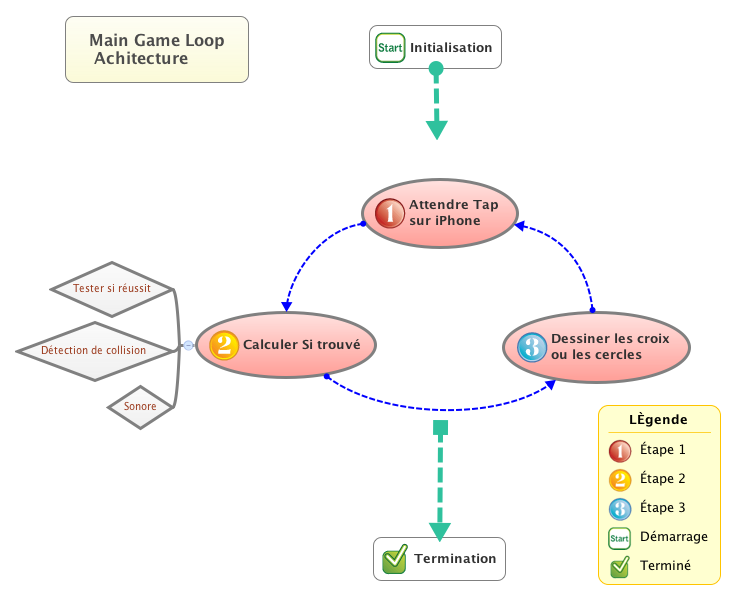
\includegraphics[width=6in]{XMinds/AchitecturePlayboy.png}
	\caption{caption}
	\label{fig:XMinds_AchitecturePlayboy}
\end{figure}
 

Nous pouvons remarquer, nous n'avons pas de module <<AI>>, <<Physics>> etc. Il nous reste que <<Tester>>, <<Détection de collision>> et <<Sonore>>. Dans l'input, il est simple aussi, ce que nous attendons est le <<tap>> sur l'écran de l'iPhone. Dans l'étape de dessiner, nous dessinons les croix si joueur s'est trompé, ou un cercle si il a trouvé une différence.

Nous n'avons pas besoins de mettre à jours cette cycle 60 fois par seconds. 

Ce jeu comporte beaucoup des autre composant de genre d'application en dehors du jeu. C-à-dire la boutique, la notification, le scoring, twitter \& facebook etc..
Je vais les parle dans le section suivante.

% subsection le_structure_de_playboy_spots_ (end)

\subsection{Le structure des système} % (fold)

<<Playboy-Spots>> comporte plusieurs composantes autour du jeu. La gros schéma suivante comme figure~\ref{fig:XMinds_PlayboySpotsApp} va décrit la structure générale du <<Playboy-Spots>>.
\begin{figure}[htbp]
	\centering
		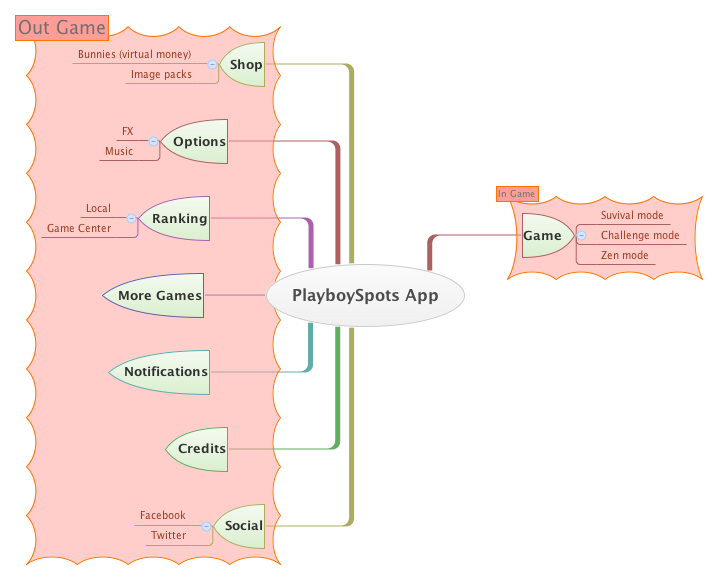
\includegraphics[width=6in]{XMinds/PlayboySpotsApp.png}
	\caption{caption}
	\label{fig:XMinds_PlayboySpotsApp}
\end{figure}



On peut remarquer que, il y a 7 composante en dehors du jeu. Il y a , shop, Options, Ranking, More Games, Notifications, Credits \& Social. Sauf le jeu, toute les autre composants sont crée par UIKit. Dans les autres composants, nous avons utilisé quand même beaucoup des bibliothèque pour faciliter notre travail, et pour obtenir un bon résultat.

\begin{description}
	\item[Shop] Shop est un UIView qui permet au joueur d'acheter les nouveaux packs, les bunnies et télécharger les nouveaux image. Y compris un fonction de <<CoverFlow>> pour améliorer l'affichage des packs.
	\item[Options] C'est un layer devant le jeu, qui fournit des options pour permettre de activer et désactiver le musique et FX effect.
	\item[Ranking] Un UIView qui permet de afficher toutes les scores local.
	\item[More Games] Un web view qui se charge d'afficher un site web de chugulu qui proposer des autres jeux du chugulu games.
	\item[Notification] Un système qui gène tous les notifications, afficher et supprimer.
	\item[Crédit] Un view simple qui afficher le crédit de l'équipe de chugulu.
	\item[Social] Un composant qui se charge de poster des scores, des phrases sur des site social comme twitter et facebook.
\end{description}


De l'autre coté, nous pouvons remarquer que nous avons 3 mode du qui sont Mode Suivival, Mode challenge et Mode zen. En réalisant toutes les composant, nous avons choisi beaucoup des bibliothèque existant. Nous n'avons pas besoins de refaire des outils qui existe, la meilleurs façons est d'essayer de trouver ce qui existe, prend-le, changer-le pour adapter nos besoins.

Le Figure~\ref{fig:XMinds_PlayboySpotsAppExternals} montre que les bibliothèques que nous avons utilisé dans <<Playboy-Spots>>. La plupart des bibliothèques sont gratuit est open-source. Nous avons quand-même une biliothèque interne, qui est utilisé par chugulu, qui est privé aussi. 

\begin{figure}[htbp]
	\centering
		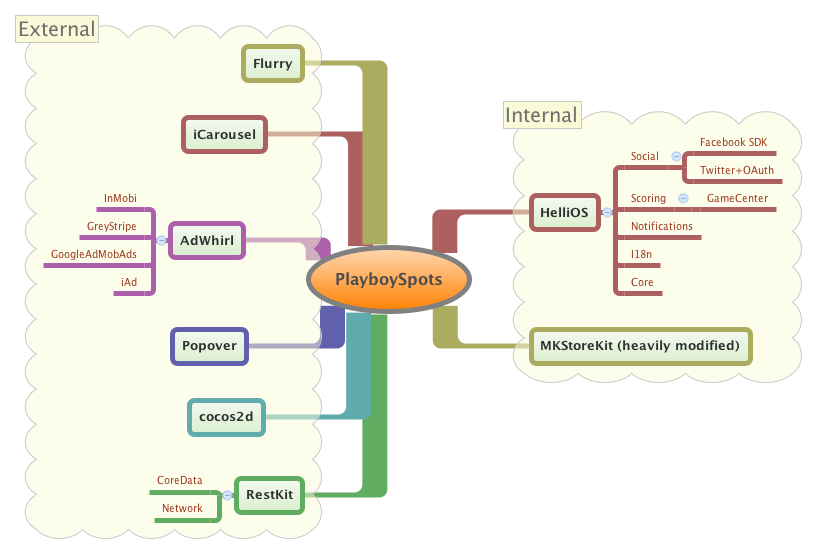
\includegraphics[width=7in]{XMinds/PlayboySpotsAppExternals.png}
	\caption{caption}
	\label{fig:XMinds_PlayboySpotsAppExternals}
\end{figure}

\begin{description}
	\item[Flurry] Une bibliothèque utilisé pour synchronisé les status des jeux avec un site web. Utilisé pour analysé les événement des joueurs. Quel heure, ce jeu est joué le plus.
	\item[iCarousel] Une bibliothèque utilisé pour afficher toutes les packs comme cover view, qui est un effect utilisé par Apple, mais privé.
	\item[AdWhirl] Une bibliothèque utilisé pour afficher les pubs
	\item[Popover] Une bibliothèque utilisé pour afficher un popover sur iPhone. Le popover n'est fournit que sur iPad par Apple.
	\item[cocos2d] Une bibliothèque trop connu du monde, utilisé pour créer des jeux en 2D sur iOS.
	\item[RestKit] Une bibliothèque très connue du monde, utilisé pour gére les communication avec un serveur de style restful.
	\item[Hellios] Une bibliothèque privé, n'utilisé que chez chugulu games
	\item[MKStoreKit] Une bibliothèque pour faciliter acheter sur App Store. Elle est modifié beaucoup pour adapter chez chugulu.
\end{description}


% subsection Le structure des système (end)


\subsection{Synchronisation CS} % (fold)

Le synchronisation de <<Playboy-Spots>> est important, parce que nous avons besoins de synchroniser notre scores avec le <<Game Center>> d'Apple, les status avec Twitter, facebook. Les informations debug avec Flurry. L'ads avec <<AdWhirl>>. Et surtout les images, les game stats, notification avec notre serveur.

En présentant dans le figure~\ref{fig:XMinds_DataFlow} suivant, nous avons toutes les Data flow du <<Playboy-Spots>>.

\begin{figure}[htbp]
	\centering
		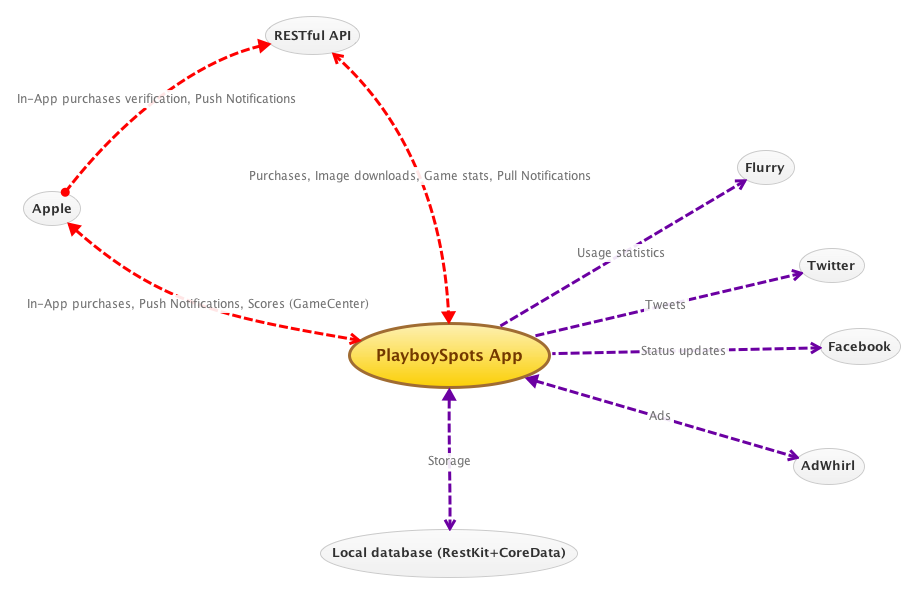
\includegraphics[width=7in]{XMinds/DataFlow.png}
	\caption{caption}
	\label{fig:XMinds_DataFlow}
\end{figure}

Les plus importants sont les synchronisation en rouge, qui supporte toute les fonctionnalités du jeu. On peut trouver les <<in-App pruchase>>, <<Push Notification>>, <<Scores>>, <<Image Download>> etc.
Nous synchronisons nos informations en utilisant le format de Json. Par une bibliothèque <<Restkit>>. Qui est très facile pour encapsuler les donnée en json et envoyer, mapping un object dans un serveur  

% subsection Synchronisation CS (end)

\subsection{La base des données} % (fold)

Le base des données est très important pour <<Playboy-Spots>>. Nous sauvegarder toutes les scores, les stats du jeu, les informations des joueur, même si les images. 
Voici le schéma de la base des données que nous utilisons dans <<Playboy-Spots>>.

% TODO add schéma de la base des donnée.


% subsection  (end)

% section structure (end)

\section{Test \& Amélioration} % (fold)
\label{sec:test_&_amélioration}

La phrase avant dernière est la phrase de <<Test\&Amélioration>>. Cette phrase est souvent très importante pour un jeu ou un logiciel. Cette phrase comporte 2 partie en parallèle, un est <<Test \& Debug>>, l'autre est <<Amélioration>>. La raison pour mettre test est amélioration dans une seule phrase, et les faire en parallèle, c'est parce que les 2 peut se effecter. Souvent, nous avons un bugue à corriger, en fait, ce bugue peut causer gros problème d'amélioration. En revanche, pour améliorer, nous devons changer quelque méthode, qui peut tomber bien sur notre bugue.

\subsection{Debug} % (fold)
\label{sub:debug}

Le debug sur iPhone peut avoir des indices à suivi. 

La première point, iPhone est un mobile. Même s'il y a simulateur de l'iPhone sur Mac OS, il n'est pas le même chose quand même. Quand nous avons rencontré un bug gras. Souvent, nous tester sur le simulateur et l'iPhone, ou autre i-Device, en faisant cela, nous pouvons augmenter notre chance à trouver ce problème. 

La deuxième point, nous pouvons utiliser XCode pour tester. Comme les autre IDE, Xcode fournit la façon pour mettre un breakpoint, suivre la command un par un. XCode peut donner le suggestion sur le bug dans la pluspart des cas. Mais pas pour toutes les situations. Par exemple, si nous avons des threads, il est presque impossible de donner les bonnes informations par XCode. 

La troisième point. Nous avons quand même un outil très important, qui s'appelle <<instruments>>. En utilisant cette outil, nous pouvons analyser notre jeu, regarder pourquoi nous avons beaucoup des mémoire consumer. Il est possible de trouver les problème de zombie par <<instruments>> aussi. Un problème de zombie est dit que, nous avons essayer d'accèser vers un objet qui est déjà releasé.

La quatrième point. Après résoudre un debug, il faut tester en utilisant un device et le simulateur. 

Pourquoi nous avons ces difficulté à trouver un bug, c'est à cause de :

\begin{itemize}
	\item Le simulateur a un mémoire infini. C'est beaucoup plus dur à produit un bug de mémoire trop chargé. Même s'il peut simuler le limit de mémoire. Mais une chose bizarre, en utilisant <<instruments>>, nous remarquons que, le simulateur ne fait pas pareil que le device. 
	\item L'architecture de simulateur est i386. Mais l'architecture de device est Armv4, Armv6. Cela veut dire que, certaine bibliothèque ne peut être utilisée dans divice, mais fonctionne très bien sur simulateur.
	\item Idem, certaine fonctionnalité ne peut être tester que sur device. Par exemple, la fonctionnalité d'app store. 
	\item Le simulateur fonctionne très vite par rapport aux device. Peut-être un algorithem trop complexe peut fonctionne très bien sur simulateur, mais pas du tout sur device. 
\end{itemize}

% subsection debug (end)

\subsection{Amélioration} % (fold)
\label{sub:amélioration}

Dans ce jeu, nous avons beaucoup de problème de fonctionnement. Nous avons mis beaucoup de temps pour améliorer notre jeu. Les améliorations comportes certaine topics comme suivantes:

\begin{itemize}
	\item Améliorer le problème de mémoire consumer. Dimunier la consumation des mémoire peut améliorer notre jeu. 
	\item Utiliser des code spécial pour certaines chose importante.
	\item Enlever les code inutile.
	\item Essayer de mettre le code en multi-thread.
	\item Cacher object qui est utilisé souvent.
	\item ...
\end{itemize}

Je vais parler principalement sur <<Multi-thread>> et <<Sérialisation>>.

\subsubsection{Multi-threading} % (fold)
\label{ssub:multi_thread}

La raison pour utiliser multi-threading, c'est pour libérer le main-thread. Si nous faisons trop de travaille dans le main-thread, il va bloquer notre applications. Parce que, le main-thread se charge d'interactiver avec le joueur. Cela veut dire que, si nous faisons trop charger le main-thread, il ne peut plus interactiver avec le joueur. 

Le façon pour résoudre ce problème est essayer de créer des threads pour des tâches qui sont lourdre. Par exemple, les tâches pour charger une photo du disque dur à mémoire est une tâche lourdre. C'est souvent dans ce jeu, car chaque fois, le joueur a trouver toutes les différence, il faut remplacer les images par des nouveaux images. Pareil pour téléchargement, nous sauvegarder toutes les données sois dans la base des données, soit dans le disque dur. N'import quelle façon va prendre beaucoup de temps. Il faut que nous fasse plusieurs thread pour chaque tâche.

Pour faire multi-thread dans l'application iPhone, nous pouvons utiliser la techniques fournit par Apple, qui s'appelle GCD, qui est abréviation de <<Grand Central Dispatch>>.

% TODO add logo GCD

Grand Central Dispatch est une technologie développée par Apple pour optimiser le support des processeurs multi-cœurs dans Mac OS X 10.6.
Cette nouvelle architecture est conçue pour permettre aux développeurs d'utiliser le potentiel des processeurs multi-cœurs. Elle travaille en distribuant efficacement les processus aux différents cœurs.
Le 11 septembre 2009, Apple a ouvert le code de Grand Central Dispatch aux contributeurs externes sous le nom de libdispatch1. Depuis, il a été annoncé que FreeBSD 8.1 prendra en charge libdispatch, ce qui laisse à penser que cette technologie pourrait être appliquée à d'autres environnements libres2.


% subsubsection multi_thread (end)

\subsubsection{Sérialisation} % (fold)
\label{ssub:sérialisation}

C'est une technique très utile. Comme pour beaucoup de choix algorithmiques, plus le mécanisme de sérialisation est spécialisé pour un type de données spécifique, plus il sera performant. Par exemple, si on ne veut transmettre que dix nombres dont les valeurs sont comprises entre 0 et 255, il suffira de 1 octet par nombre. Si par contre on ne sait pas à l'avance la quantité d'objets à transmettre on devra prévoir un ou plusieurs octets supplémentaires pour transmettre cette quantité. Si en plus ce ne sont pas seulement des nombres entiers, mais des objets quelconques que l'on souhaite transmettre, il faudra prévoir d'y associer les informations qui permettront de coder le type précis de chaque objet.

Plus globalement, il est nécessaire de faire un a priori sur les ressources disponibles au moment de la désérialisation pour déterminer les informations que l'on pourra reconstruire à l'aide d'une simple référence et celles qu'il est nécessaire d'encoder. C'est par exemple le cas des polices de caractères dans un fichier PDF : selon que l'on souhaite privilégier l'exactitude du rendu sur toutes les machines ou la taille du fichier généré, il est possible de transmettre la définition complète du tracé des caractères ou de se contenter de transmettre le nom de la police et quelques autres caractéristiques de base, en laissant le soin aux machines cibles de rechercher la police la plus adaptée parmi celles dont elle dispose.

Nous utilisons sérialisation pour nos images, en faisons cela, nous pouvons éviter de re construire les image de la base des données.
% subsubsection sérialisation (end)

% subsection amélioration (end)

% section test_&_amélioration (end)

% chapter développement_d_un_jeu (end)